\section{Perulangan Pada Python}
Perulangan dalam bahasa pemrograman berfungsi untuk memerintahkan komputer melakukan sesuatu secara berulang-ulang. Terdapat dua jenis perulangan dalam bahasa pemrograman python, yaitu perulangan dengan for dan while.
\subsection{While dan For}
Perulangan while disebut dengan uncounted loop (perulangan yang tak terhitung), sementara perulangan for disebut dengan counted loop (perulangan yang terhitung). Perbedaannya adalah ada statement while, biasanya memiliki ciri berupa pengecekan kondisi dan perulangan dilakukan diawal. Sedangkan pada statement for, memiliki ciri berupa inisialisasi perulangan dilakukan diawal statement dan perulangan tersebut akan berhenti ketika syarat/ kondisi yang telah ditentukan terpenuhi\cite{santoso2009bahasa}.

\subsection{Perintah Break, Continue dan Pass Perintah Break}
\subsubsection{Perintah Break}
Perintah break dipakai untuk menghentikan proses berjalannya iterasi atau perulangan pada statement for atau while\cite{arfian2012rekayasa}.Dan semua kode setelah pernyataan break akan segera diabaikan. Pernyataan break ini dapat kita gunakan pada pengulangan while dan for.
Statement yang berada di bawah break tidak akan di eksekusi dan program akan keluar dari proses looping.  
Contoh break : 
\begin{equation}
>>> x = 1     
>>> while x < 5:     
...    if x == 3:     
...      break     
...    print x     
...    x = x+1                                                                                                                    
... else:          
print "Loop sdh selesai dikrjkn"   
 ...     
1    
2 
\end{equation}

\subsubsection{Perintah Continue}
Perintah continue dapat dipakai untuk meloncati sebuah perulangan, maksudnya adalah intruksi yang seharusnya dapat dilewati, hal ini berarti instruksi tidak akan dijalankan\cite{arfian2012rekayasa}. pernyataan continue akan dilakukan pengulangan mulai dari awal lagi. Dan mengabaikan semua kode yang tersisa pada loop untuk menuju keawal loop lagi.
Misal:
\begin(equation}
for(int i = l; i <= 100; i++){
    if(i % 2 == 0){
        continue;
    }
    System.out.println(i);
    }
\end(equation}

Jika program tersebut dijalankan, maka hasilnya akan menampilkan angka-angka ganjil saja, hal ini disebabkan karena saat nilai i merupakan angka genap, maka statement continue akan membuat program tidak menampilkan angka genap.

\subsubsection{Perintah Pass}
Sebenarnya perintah pass tidak memiliki fungsi yang sangat penting. Dan bahkan sangat jarang digunakan oleh programmer. Jadi perintah pass ini sebenarnya hanya mengisi kekosongan saja, agar program tidak eror nantinya.perintah pass akan Menyebabkan program tidak melakukan tindakan. Digunakan untuk mengabaikan sesuatu statement perulangan, pengkodisian, class dan fungsi yang belum di definisikan badan programnya agar tidak terjadi error.
\begin{equation}
for i in range (5) :
    if i == 5 :
        pass
    print(i)
    \end{equation}

Jadi seperti yang sudah dikatakan sebelumnya, perintah pass ini memiliki fungsi untuk mengisi kekosongan dari sebuah penyeleksian ataupun perulangan.

 \subsubsection{Perintah return}
Perintah return dapat menghentikan suatu proses dari fungsi sebelum mengakhiri fungsi tersebut. Alasan menggunakan perintah return adalah jika menemui sebuah kesalahan kondisi, yang berarti nilai suatu fungsi tersebut mengembalikan nilai null (kosong) : 
import math
\begin{equation}
def print_log (x):
  if x <= 0 :
    print x, 
\"Bilangan lebih sama dengan 0\"  
  return  
hasil = math.log (x) 
 print \"Hasil log dari\", x, \"adalah\", hasil 
 \begin{equation}

\subsection{Nested Loop}
Nested Loop (Perulangan Bertingkat) adalah semua tipe perulangan yang dapat dipakai di dalam perulangan yang lain. Jadi Perulangan for bisa dipakai di dalam for yang lain, perulangan for bisa berada didalam perulangan while, perulangan while bisa dipakai di dalam perulangan while yang lain, dan perulangan while bisa di dalam perulangan for.
\subsubsection{Contoh Penggunaan Nested Loop}
Format nested loop (for di dalam for)
\begin{equation}
For iterasi_var_1 in urutan_1:
	Statements_untuk_perulangan_for_yang_di_luar
...
For iterasi_var_1 in urutan_2:
	Statements_untuk_perulangan_for_yang_di_dalam
...
Statements_untuk_perulangan_for_yang_di_luar
...
\end{equation}

Format nested loop (while di dalam while)
\begin{equation}
While expressions:
	Statements_untuk_perulangan_while_yang_di_dalam
...
Statements_untuk_perulangan_whle_yang_di_luar
...
\end{equation}

Contoh :
\begin{equation}
X = int(input(“Masukkan jumlah bariss: “))
For i in range (x) :
	For j in range(i+1):
		Print(“*”, end=””)
	Print()
\end{equation}
Saat di Run Module maka :
Masukkan jumlah bariss: 5 (inputkan 5)
*
**
***
****
***** 
Muncul 5 baris isi bintang


\subsection(While Loop)
Perintah While pada pyton biasanya memiliki ciri berupa pengecekan kondisi dan perulangan dilakukan diawal\cite{santoso2009bahasa}. Alur prosesnya adalah ketika sebuah program dijalankan dan kemudian menemukan sebuah kondisi dimana menggunakan loop atau perulangan while, jika kondisi true maka statment itu akan dieksekusi kemudian akan di cek lagi kondisinya. Setelah selesai statmentnya masih true dieksekusi lalu akan mengecek lagi kondisinya dan terus seperti itu, dan jika false statementntya maka akan keluar dari perulangan dan akan melanjutkan ke program selanjutnya.

\subsection{Perulangan do-while}
Perulangan do-while merupakan perulangan yang  mirip dengan perulangan while namun perbedaannya\cite{arfian2012rekayasa}, pada perulangan do-whiile, maka minimal instruksi akan dijalnkan sekali. Contoh statement do-while:
\begin{equation}
int jumlah = 100;
do{
    System.out.println(jumlah);
    jumlah++; // naikkan jumlah
}while(jumlah <= 10);
\end{equation}
Jika program itu dijalankan, maka akan menghasilkan keluaran 100,  yang artinya walaupun kondisinya salah, namun minimal isi instruksi akan dijalankan sekali, hal ini disebabkan karena proses do-while berbeda dengan while,  yang dimana do-while pertama melakukan instruksi setelah itu baru mengecek kondisi, sedangkan while pertama mengecek kondisi baru melakukan instruksi. 

\subsection{Perulangan (for loop)}
FOR Loop dipakai untuk melakukan perulangan atau iterasi mencapai batas atau jarak yang telah ditentukan/cite{santoso2009bahasa}.

Kegunaan
\begin{enumerate}
\item Ketika ingin pergi ke item urutan tertentu seperti pada list atau string
\item Ketika ingin melakukan perulangan kode beberapa kali
\end{enumerate}
For interaksi_var in ururan
Statements
Print(“bukan bagian perulangan”) 

\subsection{For Loop}
Perulangan for disebut juga counted loop (perulangan yang terhitung)
Pengulangan for digunakan untuk pengulangan dengan muatan yang banyak\cite{van2007python}.
keistimewaan perulanga pada for adalah , perulangan dapat di hentikan pada saat kondisi tertentu. pada python, statemen for bekerja mengulang berbagai macam tipe data sekuensial seperti pada list, string dan tuple
Contohnya Seperti :
\begin{equation}
for a in range(0, 10):
	print a
\end{equation}
Hasil Outputnya :
\begin{equation}
python for.py
0
1
2
3
4
5
6
7
8
9
\end{equation}


\subsection{While Loop}
perulangan while disebut juga uncounted loop (perulangan yang tak terhitung)
Pengulangan while biasanya digunakan untuk sesuatu yang ga pasti.
Contohnya Seperti :
\begin{equation}
a = 0
while true:
	if a < 10:
		print "saat ini a bernilai: ", a
		a = a + 1
	else a >= 5:
		break
\end{equation}
Hasil Outputnya :
\begin{equation}
python while.py
saat ini a bernilai: 0
saat ini a bernilai: 1
saat ini a bernilai: 2
saat ini a bernilai: 3
\end{equation}

\subsection{For looping with list}
Contohnya Seperti :
\begin{equation}
hero_dota2_character = ["Mirana", "Axe", "Tusk"]
for character in hero_dota2_character:
	print character
\end{equation}
Hasil Outputnya :
\begin{equation}
python for-list.py
Mirana
Axe
Tusk
\end{equation}

\subsection{break and continue statements}
Jeda digunakan untuk for loop atau while loop, sedangkan terus digunakan untuk melewati blok saat ini, dan kembali ke pertanyaan for atau while.
Contoh pertama seperti :
\begin{equation}
count = 0
while True:
    print(count)
    count += 1
    if count >= 5:
        break
		\end{equation}
Output pertama :
\begin{equation}
python while.py
0
1
2
3
4
\end{equation}

\subsection{Range}
\subsubsection{Fungsi range()}
Jika ingin melakukan perulangan dengan sejumlah yang diinginkan, fungsi built-in range sangat membantu. Fungsi tersebut menghasilkan sejumlah indeks dari nilai yang telah ditentukan. 
Contohnya :
\begin{equation}
>>> range(15)
[0, 1, 2, 3, 4, 5, 6, 7, 8, 9, 10, 11, 12, 13, 14]
Ataupun sebagian angka yang diinginkan. Contohnya :
>>> range (8, 15)
[8, 9, 10, 11, 12, 13, 14]
>>> range(0,9,3)
[0, 3, 6]
>>> range(0, 20, 3)
[0, 3, 6, 9, 12, 15, 18]
\end{equation}
 Contoh tersebut menunjukan kelipatan dari suatu interval bilangan yang mempunyai sintaks range(<nilai-awal>, <nilai-akhir>, <kelipatan-angka>).
\subsubsection{Contoh penggunaan range(nilai_awal,nilai_akhir,pencacah)}
Berikut ini contoh penggunaan range untuk menampilkan bilangan dari 1 – 100 dengan penambahan/pencacah 1 dengan menambahkan end=’ ’ agar bilangan tampil secara horizontal tidak pindah baris ke bawah
\begin{equation}
for i in range(1, 101, 1) :
    print(i, end=' ')
\end{equation}
Lalu, setelah perintah diatas dijalankan (run) maka akan tampil bilangan seperti berikut ini :
\ref{2_range}

\begin{figure}[ht]
    \centerline{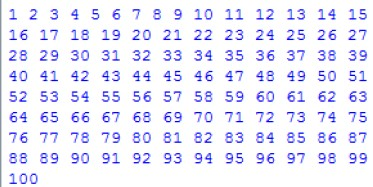
\includegraphics[width=1\textwidth]{figures/2_range.JPG}}
    \caption{hasil penggunaan range}
    \label{2_range}
    \end{figure}

\subsection{for loop with else}
For loop bisa memiliki blok else yang opsional juga. Bagian lain dijalankan jika item urutan digunakan dalam lingkaran for loop .
Pernyataan break bisa digunakan untuk menghentikan sebuah loop. Dalam kasus seperti itu, bagian yang lain diabaikan.

Oleh karena itu, bagian loop yang lain berjalan jika tidak terjadi pemutusan.

Berikut adalah contoh untuk menggambarkan hal ini.
\begin{equation}
script.py 
digits = [0, 1, 5]

for i in digits:
    print(i)
else:
    print("No items left.")
Output :
0
1
5
No items left.
\end{equation}
